% ==========================
%  LaTeX 2e - Dokument
%  Editor: Dragan Kozulovic
% ==========================
\documentclass[11pt,a4paper,fleqn,twoside]{report}
\usepackage[dvips,final]{graphicx}               %% epsfig 
\usepackage[utf8]{inputenc}                    %% ISO-Text 
\usepackage[T1]{fontenc}                         %% 
\usepackage[german]{babel}                       %% BABEL 
\usepackage{parskip}                             %% 
\usepackage{fancyhdr}                            %% 
\usepackage[hang,bf]{caption}                    %% 
\usepackage{color}                               %% Farben
\usepackage{multirow}                            %% 
\usepackage{natbib}
\usepackage{float}

\usepackage{amsmath}
\usepackage{graphicx}
\usepackage[onehalfspacing]{setspace}
%\usepackage[flushleft]{threeparttable}
\usepackage{blindtext}
\usepackage{amssymb}
%\usepackage{esvect}
%\usepackage[breaklinks]{hyperref} 



% Einzubindende Dateien 
\includeonly{Titelseite,
             Letzte_Seite,
	     eid_erkl,
	     Nomenklatur}
\graphicspath{{Bilder/}}                         %% Pfad fuer einzubindende Graphiken


% Seiten-Layout
\oddsidemargin   0.0cm                           %% Anpassung DIN A4-Format (symmetrisch)
\evensidemargin  0.0cm                           %% Anpassung DIN A4-Format (symmetrisch)
\topmargin      -1.0cm         
\textheight     25.0cm
\textwidth      16.0cm
\pagestyle{fancy}
\renewcommand{\chaptermark}[1]{\markboth{\thechapter.\ #1}{}}
\renewcommand{\sectionmark}[1]{\markright{\thesection\ #1}}
\fancyhf{}                                %Clears all header and footer fields, in preparation.
\fancyhead[LE,RO]{\thepage}               %Displays the page number in bold in the header,
                                          % to the left on even pages and to the right on odd pages.
\fancyhead[RE]{\nouppercase{\leftmark}}   %Displays the upper-level (chapter) information---
                                          % as determined above---in non-upper case in the header, to the right on even pages.
\fancyhead[LO]{\rightmark}                %Displays the lower-level (section) information---as
                                          % determined above---in the header, to the left on odd pages.
\renewcommand{\headrulewidth}{0.5pt}      %Underlines the header. (Set to 0pt if not required).

%\sloppy                                         %% lockerer Zeilenumbruch
%\flushbottom                                    %% buendige letzte Zeile


% Trennungskorrekturen
%\hyphenation{Bei-spiel}
%\hyphenation{}
%\hyphenation{}
%\hyphenation{}
%\hyphenation{}
%\hyphenation{}


% Umbenennungen (babel) (siehe LaTeX-Begleiter, Abschn. 9.2.3)
\addto\extrasgerman{\renewcommand{\figurename}{Abb.}}


% Listen
\newcommand{\bl}{\begin{list}{\textbullet}%         %% kleine Aufzaehlung/Liste
{\topsep0pt\partopsep0pt\itemsep0pt\parsep0pt\leftmargin1.5em\labelwidth1em\labelsep0.5em}}
\newcommand{\el}{\end{list}}
\newcommand{\cit}[1]{\textit{\cite{#1}}}




\begin{document}
% Titelseite
\begin{titlepage}
 \centering

\begin{table}[htbp]
 \begin{center}
 \vspace{-0.5cm}
% \renewcommand{\arraystretch}{1.5}
  \begin{tabular}{lcr} 
    \parbox{0.45\textwidth}{\mbox{ }} & \parbox{0.13\textwidth}{\mbox{ }} & \parbox{0.45\textwidth}{\mbox{ }} \\
    \hspace*{-2.0cm}
    
\includegraphics[width=0.42\textwidth]{./Bilder/TUBraunschweig_4C.pdf} &		 					\includegraphics*[width=0.5\textwidth]{./Bilder/iff_logo_v007.pdf} 
       \\ %empty
  \end{tabular}
 \end{center}
\end{table}


 \vspace*{2.0cm}

 \textbf{\large Protokoll}


 \vspace*{1.5cm}
 
 \textbf{\LARGE Überschrift} \\[0.5ex]


 \vspace*{1.5cm}
 
 \textbf{\large Nico Hempen} \\[0.5ex]
 \textbf{Matrikelnummer 4753519}
 
 \textbf{\large Finn Matz} \\[0.5ex]
 \textbf{Matrikelnummer 4810384}
 
 \textbf{\large -} \\[0.5ex]
 \textbf{Matrikelnummer -------}
 
 \textbf{\large -} \\[0.5ex]
 \textbf{Matrikelnummer -------}
 
 \textbf{\large -} \\[0.5ex]
 \textbf{Matrikelnummer -------}
 

 

 



 \vspace*{2.5cm}

 \begin{table}[htbp]
  \begin{center}
%  \renewcommand{\arraystretch}{1.5}
   \begin{tabular}{rl} 
     \parbox{0.33\textwidth}{\mbox{ }} & \parbox{0.66\textwidth}{\mbox{ }} \\
     Ausgegeben: & Institut f\" ur Flugf\" uhrung \\
                 & Institutsleiter: Prof. Dr. P. Hecker \\
                 & Technische Universit\" at Braunschweig \\
                 &  \\
       Betreuer: & -\\
 %(Erstellt bei:) & (Externe Firma, Stadt) \\
                 %&  \\
 Ver"offentlichung: & Datum \\
   \end{tabular}
  \end{center}
 \end{table}



\end{titlepage}


%only blank page
\newpage
\thispagestyle{empty}
\mbox{}


\pagenumbering{roman}\setcounter{page}{1} 


%% Eidesstattliche Erklaerung (fuer DA, MA und BA)
\chapter*{Eidesstattliche Erkl"arung}\label{s:eid_erkl}


Hiermit erkl"are wir, -, -, -, - und - des Eides statt, das vorliegende Protokoll selbstst"andig und ohne
fremde Hilfe verfasst und keine anderen als die angegebenen Hilfsmittel verwendet zu
haben.

\vspace*{3cm}
Braunschweig, Datum

%\include{empty_page}


% Uebersicht
%\include{abstract}
%\include{empty_page}


% Inhaltsverzeichnis
\fancyhead[RE]{Inhaltsverzeichnis}
\fancyhead[LO]{Inhaltsverzeichnis}
{ 
   \renewcommand{\baselinestretch}{0.85}    %% Zeilenabstand / TOC
   \small\normalsize                        %% neuen Zeilenabstand aktivieren
   \tableofcontents
}
% ATTENTION: comment out if contents sides are even number
%\include{empty_page}


% Nomenklatur
\newpage
\fancyhead[RE]{Nomenklatur}
\fancyhead[LO]{Nomenklatur}
\chapter*{Nomenklatur}
\addcontentsline{toc}{chapter}{Nomenklatur}



\subsection*{Griechische Bezeichnungen}
\begin{tabbing}
\hspace*{2cm}\=\kill
$\alpha$ \> Anstellwinkel \\[0.2ex]
$\gamma$ \> Bahnneigungswinkel \\[0.2ex]
$\eta$ \> Trimmwinkel \\[0.2ex]
$\epsilon_{min}$ \> minimale reziproke Gleitzahl \\[0.2ex]
$\Lambda$ \> Flügelstreckung \\[0.2ex]
$\kappa$ \> Isentropenkoeffizient \\[0.2ex]
$\rho$ \> Luftdichte \\[0.2ex]
\end{tabbing}


\subsection*{Formelzeichen}
\begin{tabbing}
\hspace*{2cm}\=\kill
$A$ \> Auftrieb \\[0.2ex]
$C_A$ \> Auftriebsbeiwert \\[0.2ex]
$C_A^*$ \> Auftriebsbeiwert bei $\epsilon_{min}$ \\[0.2ex]
$C_{A \alpha}$ \> Auftriebsanstieg \\[0.2ex]
$C_W$ \> Widerstandsbeiwert \\[0.2ex]
$C_{W0}$ \> Nullwiderstandsbeiwert \\[0.2ex]
$C_W^*$ \> Widerstandsbeiwert bei $\epsilon_{min}$ \\[0.2ex]
$G$ \> Gewicht \\[0.2ex]
$g$ \> Erdbeschleunigung \\[0.2ex]
$H$ \> Flughöhe \\[0.2ex]
$k$ \> Widerstandsanstieg \\[0.2ex]
$\mathrm{k}$ \> k-Faktor \\[0.2ex]
$m$ \> Masse \\[0.2ex]
$p$ \> Luftdruck \\[0.2ex]
$q$ \> Staudruck \\[0.2ex]
$R$ \> Gaskonstante \\[0.2ex]
$T$ \> Temperatur \\[0.2ex]
$t$ \> Zeit \\[0.2ex]
$V_{IAS}$ \> angezeigte Fluggeschwindigkeit \\[0.2ex]
$V_{TAS}$ \> wahre Fluggeschwindigkeit \\[0.2ex]
$V_{opt}$ \> Fluggeschwindigkeit beim besten Gleiten \\[0.2ex]
$W$ \> Widerstand \\[0.2ex]
$W_{min}$ \> minimaler Widerstand \\[0.2ex]
\end{tabbing}



% alle Kapitel
\pagenumbering{arabic}\setcounter{page}{1}
\fancyhead[RE]{\nouppercase{\leftmark}}
\fancyhead[LO]{\rightmark}

\chapter{Einleitung (VR)}
\label{c:Einleitung}

tbd




\begin{table}[h]
	\centering
	\begin{tabular}{lr}
		
		Name & \hspace{0.5cm} Initialen\\
		\hline
		Nico Hempen & NH\\
		Tim Gotzel & TG\\
		Finn Matz & FM\\
		Alexander Göhmann & AG \\
		Viktor Rein & VR\\
		\hline
		
	\end{tabular}
	\caption{Initialen der beteiligten Personen}
	\label{tab:initialien}
\end{table}

\chapter{Theoretische Grundlagen (NH)(FM)}
\label{c:TheoGrund}

\section{Luftdichte $\rho$}

Zur Bestimmung der real vorherrschenden Luftdichte in der gegebenen Höhe, wird unter der Annahme, dass Luft ein ideales Gas ist, diese Luftdichte mit der Idealen Gasgleichung definiert:

\begin{equation}
\rho_{real}=\frac{m}{V}=\frac{p}{R_{Luft} \cdot T}
\end{equation}

Dabei kann $R_{Luft}=\SI{287,058 }{\ \joule\kilogram^{-1}\kelvin^{-1}}$ gesetzt werden und der Luftdruck $p$ in definierter Höhe über die Temperatur $T$ mittels der Isentropenbeziehung berechnet werden:

\begin{equation}
p=\left(\frac{T}{T_0}\right)^{\frac{\kappa}{\kappa-1}} \cdot p_0
\end{equation}

Dabei gilt für die Standardbedingungen $T_0=\SI{288,15}{\ \kelvin}$ und $p_0=\SI{101300}{\ \pascal}$.

\section{Wahre Fluggeschwindigkeit $V_{TAS}$}

In den von uns aufgezeichneten Daten der DO-128, sowie in den bereitgestellten Daten der DO-28, liegt die Information der Fluggeschwindigkeit lediglich als \textit{indicated airspeed} vor. Zur Bestimmung der nachfolgenden Beiwerte und Zusammenhänge zwischen den Kenngrößen ist jedoch die so genannte \textit{true airspeed} von Bedeutung. Zur Bestimmung von $V_{TAS}$ aus $V_{IAS}$ wird folgende Formel verwendet\cite{Kurzskript}:

\begin{equation}
V_{TAS}=\sqrt{\frac{\rho_0}{\rho_{real}} \cdot V_{IAS}^2}
\end{equation}

Dabei kann $\rho_0$ als Luftdichte zu $\SI{1,225}{\ \kilogram\meter^{-3}}$ gesetzt werden. Die Fluggeschwindigkeit $V_{IAS}$ muss bei dem Flugversuch mit der DO-128 allerdings noch von $kn$ in $\frac{m}{s}$ umgerechnet werden:

\begin{equation}
V\left(\frac{m}{s}\right)=0,51444 \cdot V\left(kn\right)
\label{eq:V_Umrechnung}
\end{equation}


\section{Auftriebsbeiwert $C_A$}
\label{sec:CA}

Der Auftriebsbeiwert $C_A$ kann per Definition mittels folgender Gleichung bestimmt werden\cite{Skript}:

\begin{equation}
C_A=\frac{A}{\frac{\rho_{real}}{2} \cdot S \cdot V_{TAS}^2}
\label{eq:CA}
\end{equation}

Darin kann der Auftrieb $A$ über die Gewichtskraft $G$ nach folgender Gleichung aufgestellt werden:

\begin{equation}
A=\cos(\gamma) \cdot G
\label{eq:A}
\end{equation}

Da der Bahnneigungswinkel $\gamma$ lediglich in der Messreihe für die DO-28 gegeben ist, muss dieser Wert für die Messreihe der DO-128 über die Sinkgeschwindigkeit $w_{g_{real}}$ und der Fluggeschwindigkeit $V_{TAS}$ bestimmt werden:

\begin{equation}
\gamma=\arcsin\left(\frac{w_{g_{real}}}{V_{TAS}}\right)
\label{eq:gamma}
\end{equation} 

Dabei wird die Sinkgeschwindigkeit $w_{g_{real}}$ bestimmt durch\cite{Kurzskript}:

\begin{equation}
w_{g_{real}}=\frac{\Delta H_{INA}}{\Delta t} \cdot \frac{T_{real}}{T_{INA}}
\end{equation}

Worin $T_{INA}$ für die jeweiligen Höhen aus Tabellen bestimmt werden können und die übrigen Werte im Versuch aufgezeichnet wurden.

Die Flügelfläche $S$ kann in Gleichung \ref{eq:CA} durch die jeweiligen Daten der beiden Flugzeuge ersetzt werden.

\section{Widerstandsbeiwert $C_W$}

Ähnlich wie die Bestimmung des Auftriebsbeiwertes kann auch der Widerstandsbeiwert $C_W$ bestimmt werden:

\begin{equation}
C_W=\frac{W}{\frac{\rho_{real}}{2} \cdot S \cdot V_{TAS}^2}
\end{equation}

Der einzige Unterschied zu $C_A$ besteht in der Verwendung vom Widerstand $W$ statt des Auftriebs $A$ in dieser Gleichung. Dieser kann über die selbe Beziehung wie in Gleichung \ref{eq:A} bestimmt werden:

\begin{equation}
W=\sin(\gamma) \cdot G
\end{equation}

Dabei kann der Bahnneigungswinkel $\gamma$ ebenfalls mit Gleichung \ref{eq:gamma} berechnet werden.

\section{Minimaler Widerstand $W_{min}$}

Durch Auftragen des Auftriebsbeiwertes $C_A$ über den Widerstandsbeiwert $C_W$ lassen sich zum einen der Nullwiderstandsbeiwert $C_{W0}$ und zum anderen die beste Gleitzahl $C_A^*$ bestimmen. $C_{W0}$ ist der Widerstandsbeiwert beim Nullauftrieb, also bei $C_A=0$. $C_A^*$ erhält man durch Anlegen einer Tangente, die durch den Ursprung geht. Der Berührungspunkt dieser Tangente mit der Polaren, ist der Punkt des besten Gleitens. Aus diesen beiden Kennwerten lässt sich der minimale Widerstand $W_{min}$ bestimmen:

\begin{equation}
W_{min}=\frac{2 \cdot C_{W0} \cdot G}{C_A^*}
\label{eq:W_min}
\end{equation}

\section{Optimale Fluggeschwindigkeit $V_{opt}$}

Mit dem bestimmten $C_A^*$ lässt sich zusätzlich die optimale Fluggeschwindigkeit bestimmen, also die Geschwindigkeit, bei der der Widerstand am geringsten ist.

\begin{equation}
V_{opt}=\sqrt{\frac{G}{\frac{\rho}{2} \cdot S \cdot C_A^*}}
\label{eq:V_opt}
\end{equation}




\chapter{Versuchsdurchführung (TG)}
\label{c:VdurchF}

In diesem Kapitel wird die Versuchsdurchführung für den Flug mit der DO128 der Technischen Universität Braunschweig beschrieben. 

Der Flug wurde am 20.05.2019 mit 6 Mann Besatzung durchgeführt und dauerte 20 Minuten. Die vorherrschenden Umweltparameter am Boden wurden notiert und sind in Tabelle \ref{tab:VersuchDaten1} festgehalten. 


\begin{table}[h]
	\centering
	\begin{tabular}{| l | l | }
\hline
	Datum  & 20.05.2019 \\ \hline
	Beginn Flug & 9:47 \\ \hline
	Ende Flug & 10:10 \\ \hline
	Besatzung (Masse) & 461 kg \\ \hline
	Höhenmessereinstellung & 1013,25 hPa QNH \\ \hline
	Rüstmasse & 1388 kg \\ \hline
	Kraftstoffmasse am Boden & 1361 lbs \\ \hline
	Wetter & sonnig, leichte Quellwolken \\ \hline
	Temperatur  & \SI{19}{\celsius} \\ \hline
	Wind & 5 kn / 060 \\ \hline
	Druck (Platzhöhe)  & 1004 hPa  \\ \hline
	\end{tabular}
	\caption{Parameter am Versuchstag}
	\label{tab:VersuchDaten1}
\end{table}

Nach dem Einstellen des Höhenmessers auf QNH startete die DO 128 und nahm ihre Zielhöhe knapp über 4000 ft ein. Für die Versuche wurden 4 Sinkflüge bei verschiedenen Fluggeschwindigkeiten (80 kn, 100 kn, 120 kn, 140 kn) absolviert. Dabei beschleunigte der Pilot das Flugzeug auf die Sollgeschwindigkeit. Beim erreichen der 4000 ft Marke stoppte der Copilot die Zeit die benötigt wurde, um 1000 ft zu sinken, mit der Stoppuhr. Dabei wurden am Ende und am Anfang die Temperaturen und die verbrauchte Treibstoffmasse auf der 4000 ft Marke und auf der 3000 ft Marke von dem Copiloten abgelesen. Alle relevanten Daten wurden vom Copiloten per Mikro an die Besatzung weitergegeben, welche diese in die vorbereiteten Versuchsprotokolle notierte. Die Werte sind in Tabelle \ref{tab:VersuchDaten2} zu sehen. Nachdem ein Sinkflug absolviert war, stieg die DO 128 wieder auf knapp über 4000 ft und ein erneuter Sinkflug wurde eingeleitet. 


\begin{table}[H]
	\centering
	\begin{tabular}{| l | l | l | l | l | }
\hline
	Sinkflug & 1 & 2 & 3 & 4 \\ \hline
	$H_A$ [ft] & 4000 & 4000 & 4000 & 4000 \\ \hline
	$H_E$ [ft]  & 3000 & 3000 & 3000 & 3000 \\ \hline
	$T_A$  \SI{}{\celsius} & 12 & 12 & 12 & 12 \\ \hline
	$T_E$  \SI{}{\celsius} & 13 & 13 & 13 & 13 \\ \hline
	$V_{IAS}$ [kn] & 80 & 100 & 120 & 140 \\ \hline
	$m_a$ [lbs] & 237 & 262 & 284 & 304 \\ \hline
	$m_e$ [lbs] & 244 & 267 & 288 & 306 \\ \hline
	$\Delta$ t [s] & 95 & 67 & 48 & 31 \\ \hline
\end{tabular}
	\caption{Versuchsdaten}
	\label{tab:VersuchDaten2}
\end{table}

Bei dem Sinkflug handelte es sich um einen Gleiten bei verschiedenen Fluggeschwindigkeiten. Die Propeller der DO-128 lieferten nur so viel Schub, um  die Verluste zu kompensieren, die sie selber erzeugten.

\chapter{Massenabschätzung (AG)}
\label{c:Mabsch}
\chapter{Auswertung und Umrechung der Messdaten}
\label{c:Auswertung}

Messwerte vom Flugversuch mit der Do 128: 

\begin{table}[h]
	\centering
	\begin{tabular}{| l | l | l | l | l | }
\hline
	Do 128 & 1. Sinkflug & 2. Sinkflug & 3. Sinkflug & 4. Sinkflug \\ \hline
	$H_A\ [ft]$ & 4000 & 4000 & 4000 & 4000 \\ \hline
	$H_E\ [ft]$  & 3000 & 3000 & 3000 & 3000 \\ \hline
	$T_A\ [^\circ\text{C}]$  & 12 & 12 & 12 & 12 \\ \hline
	$T_E\ [^\circ\text{C}]$  & 13 & 13 & 13 & 13 \\ \hline
	$V_{IAS}\ [kn]$ & 80 & 100 & 120 & 140 \\ \hline
	$m_a\ [lbs]$ & 237 & 262 & 284 & 304 \\ \hline
	$m_e\ [lbs]$ & 244 & 267 & 288 & 306 \\ \hline
	$\Delta t\ [s]$ & 95 & 67 & 48 & 31 \\ \hline
\end{tabular}
	\caption{Versuchsdaten}
	\label{tab:VersuchDaten2}
\end{table}
Die Werte in der Tabelle werden nun so umgerechnet das sie für die folgenden Berechnungen verwendet werden können.\\
Umrechnen von Masse und Temperatur in SI-Einheiten:\\

%\ref{{eq:V_Umrechnung}\\

$T_{[^\circ\text{C}]}+273,15=T_{[K]}$\\
$m_{[lbs]}*0,4536=m_{[kg]}$\\

Umrechnen von $H_{INA}$ in $H_{real}$:\\
Berechnen des Luftdrucks:\\
$p_A=(\frac{T_A}{T_B})^ {\frac{k}{k-1}}*p_0$\\
Mit $T_{Boden}=292,15\ K;\ k=1,4;\ p_0=100400\ Pa$.\\
Berechnen der Luftdichte:\\
$\rho_{real}=\frac{p_A}{R*T_A}$\\
Mit $R=287,058\ Jkg^{-1}K^{-1}$.\\
Berechnen der tatsächlich Höhe:\\
$H_{real}=H_{INA}*\left(\frac{\rho _{INA}}{\rho _{real}}\right) $\\
Mit $\rho_{INA}=1,225\ kgm^{-3}$ und den gemessenen Höhen in Metern, umgerechnet mit
$H_{[ft]}*0,3048=H_{[m]} $.\\
%mit $\rho _{INA}=1,225\ kgm^{-3}$ und $\rho _{real 4000}=1,\ kgm^{-3}$ und  $\rho _{real 3000}=1,225\ kgm^{-3}$

Die Umrechnung von $V_{IAS_{[kn]}}$ in $V_{TAS_{[ms^{-1}]}}$ wird in den theoretischen Grundlagen \ref{c:TheoGrund} erklärt.
%$V_{[kn]}*0,5144=V_{[ms^{-1}]}$\\
%$V_{TAS_A} = \sqrt{V_{IAS}^2*\frac{\rho_0}{\rho_{real_A}}}$\\
%$V_{TAS_E} = \sqrt{V_{IAS}^2*\frac{\rho_0}{\rho_{real_E}}}$\\
%$V_{TAS} =(V_{TAS_A}+V_{TAS_E})/2$\\
%$\rho_{real}=\frac{p}{R_{Luft} \cdot T}$\\
%mit $\rho_0=1,225\ kgm^{-3}$\\

Umgerechnete Messwerte:

\begin{table}[h]
	\centering
	\begin{tabular}{| l | l | l | l | l | }
\hline
	Do 128 [SI] & 1. Sinkflug & 2. Sinkflug & 3. Sinkflug & 4. Sinkflug \\ \hline
	$H_{real_A}\ [m]$ & 1325,2 & 1325,2 & 1325,2 & 1325,2 \\ \hline
	$H_{real_E}\ [m]$  & 985,2 & 985,2 & 985,2 & 985,2 \\ \hline
	$T_A\ [K]$  & 285,15 & 285,15 & 285,15 & 285,15 \\ \hline
	$T_E\ [K]$  &  286,15 & 286,15 & 286,15 & 286,15 \\ \hline
	$V_{TAS}\ [ms^{-1}]$ & 42,82 & 53,52 & 64,23 & 74,93 \\ \hline
	$m_a\ [kg]$ & 107,50 & 118,84 & 128,82 & 137,89 \\ \hline
	$m_e\ [kg]$ & 110,68 & 121,11 & 130,63 & 138,80 \\ \hline
	$\Delta t\ [s]$ & 95 & 67 & 48 & 31 \\ \hline
\end{tabular}
	\caption{Versuchsdaten in SI-Einheiten}
	\label{tab:VersuchDaten3}
\end{table}

Daten aus der Messreihe der Do 28:\\
Der Staudruck wurde mit $q_{[mBar]}*100=q_{[Pa]}$ umgerechnet.\\

\begin{table}[h]
\begin{tabular}{|l|l|l|l|l|l|l|l|l|}
\hline
Do 28                     & \multicolumn{2}{l|}{1. Sinkflug} & \multicolumn{3}{l|}{2. Sinkflug} & \multicolumn{2}{l|}{3. Sinkflug} & 4. Sinkflug \\ \hline
Nummer & 1               & 2              & 3         & 4         & 5        & 6               & 7              & 8           \\ \hline
$H_A\ [m]$              & 1250            & 875            & 1900      & 1375      & 1000     & 1525            & 700            & 1250        \\ \hline
$H_E\ [m]$              & 1000            & 775            & 1500      & 1150      & 750      & 875             & 500            & 850         \\ \hline
$q\ [pa]$ (gemittelt)    & 19500           & 16900          & 13300     & 10500     & 7600     & 24000           & 7000           & 28000       \\ \hline
$\alpha\ [^\circ]$  (gemittelt) & 4,0             & 5,0            & 7,8       & 9,8       & 15       & 3               & 17,9           & 2,75        \\ \hline
$\eta\ [^\circ]$ (gemittelt)   & -0,6            & -0,7           & -2,5      & -3,1      & -8,1     & 0               & -10,5         & 0,25        \\ \hline
$t\ [s]$                 & 53              & 83             & 63        & 56        & 80       & 101             & 55             & 30          \\ \hline
\end{tabular}
\caption{Messreihe Do 28}
	\label{tab:VersuchDaten4}
\end{table}

\chapter{Darstellung der Ergebnisse}
\label{c:Ergebnisse}

\section{Daten zum Flugversuch der DO-128}

\subsection{Auftriebsbeiwert $C_A$ über Widerstandsbeiwert $C_{W}$}

\begin{figure}[H]
	\centering	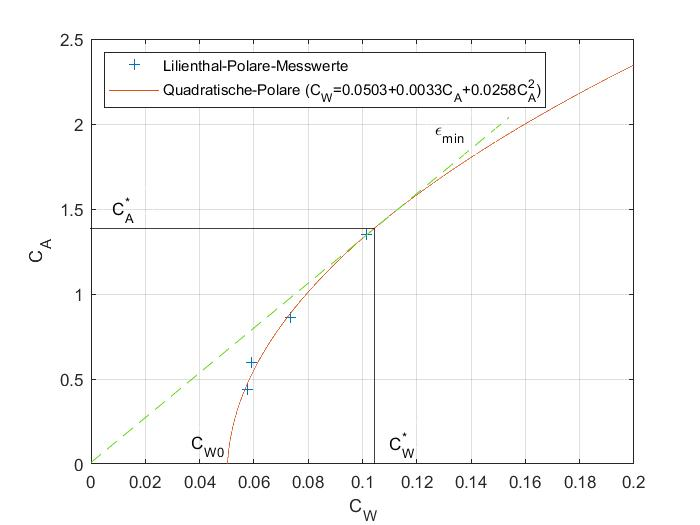
\includegraphics[width=0.7\textwidth]{./Bilder/CA_CW_DO128_NEU.jpg}
	\caption{$C_{A}$ über $C_{W}$ der DO-128}
	\label{fig:CA_CW_DO128}
\end{figure}

\subsection{Widerstand $W$ über Fluggeschwindigkeit $V$}
\label{ss:W_V}

\begin{figure}[H]
	\centering	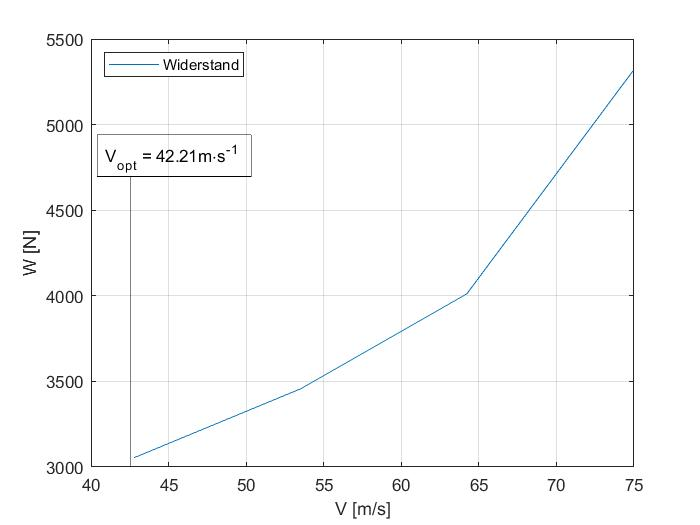
\includegraphics[width=0.7\textwidth]{./Bilder/W_V_DO128_NEU.jpg}
	\caption{$W$ über $V$ der DO-128}
	\label{fig:W_V_DO128}
\end{figure}

Die optimale Fluggeschwindigkeit $V_{opt}$ wurde, wie auch der minimale Widerstand $W_{min}$ (Im Graph nicht zu sehen), mittels der beiden Gleichungen \ref{eq:V_opt} und \ref{eq:W_min} definiert. Dazu wurde die Masse bzw. die Gewichtskraft $G$ des Flugzeugs, sowie die Dichte $\rho$ über die vier Flugabschnitte zu \SI{4142}{\ \kilogram} bzw. \SI{40633}{\ \newton} und 1,13 \SI{}{\kilogram\ \meter^{-3}} gemittelt.

\section{Daten zum Flugversuch der DO-28}

\subsection{Anstellwinkel $\alpha$ über Bahnneigungswinkel $\eta$}

\begin{figure}[H]
	\centering	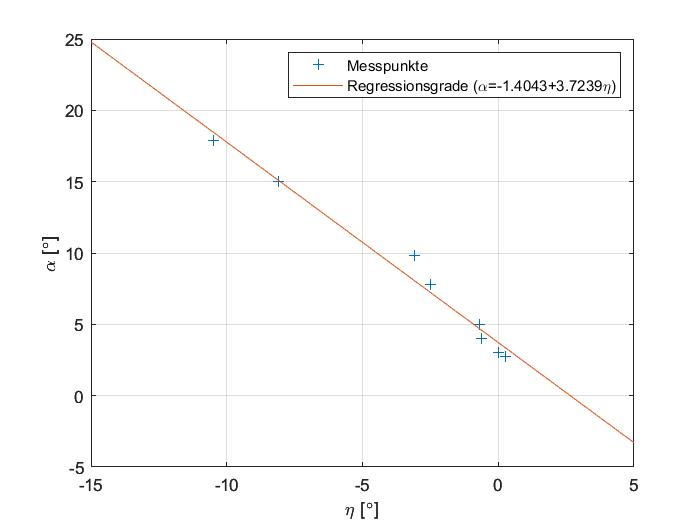
\includegraphics[width=0.7\textwidth]{./Bilder/alpha_eta_plot.jpg}
	\caption{$\alpha$ über $\eta$ der DO-28}
	\label{fig:alpha_eta_DO28}
\end{figure}

\subsection{Auftriebsbeiwert $C_{A}$ über Anstellwinkel $\alpha$}

\begin{figure}[H]
	\centering	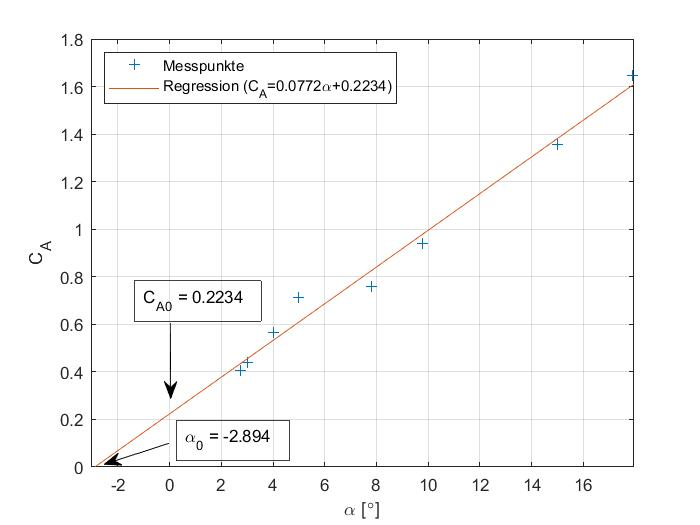
\includegraphics[width=0.7\textwidth]{./Bilder/CA_alpha_plot.jpg}
	\caption{$C_{A}$ über $\alpha$ der DO-28}
	\label{fig:CA_alpha_DO28}
\end{figure}

\subsection{Auftriebsbeiwert $C_{A}$ über Widerstandsbeiwert $C_{W}$}

\begin{figure}[H]
	\centering	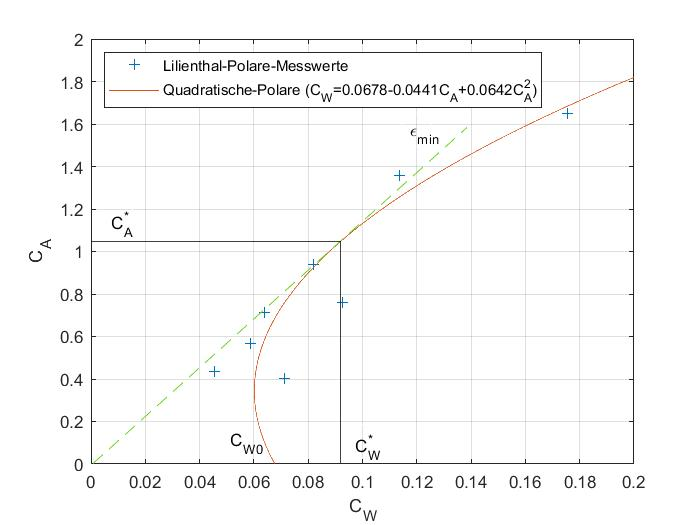
\includegraphics[width=0.7\textwidth]{./Bilder/CA_CW_DO28_NEU.jpg}
	\caption{$C_{A}$ über $C_{W}$ der DO-28}
	\label{fig:CA_CW_DO28}
\end{figure}

\subsection{Widerstand $W$ über Fluggeschwindigkeit $V$}

\begin{figure}[H]
	\centering	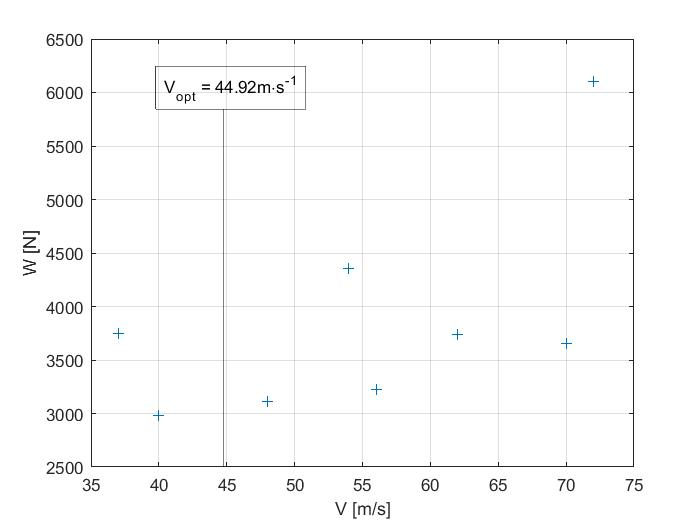
\includegraphics[width=0.7\textwidth]{./Bilder/W_V_DO28_NEU.jpg}
	\caption{$W$ über $V$ der DO-28}
	\label{fig:W_V_DO28}
\end{figure}

Äquivalent zu Abschnitt \ref{ss:W_V} wurde hier $V_{opt}$ und $W_{min}$ mittels der Gleichungen \ref{eq:V_opt} und \ref{eq:W_min} bestimmt. Dabei wurde $G$ und $\rho$ aus den 8 Flugabschnitten gemittelt zu \SI{35728}{\ \newton} und 1,21 \SI{}{\kilogram\ \meter^{-3}}.

\subsection{Fluggeschwindigkeit $V$ und Staudruck $q$ über Anstellwinkel $\alpha$}

\begin{figure}[H]
	\centering	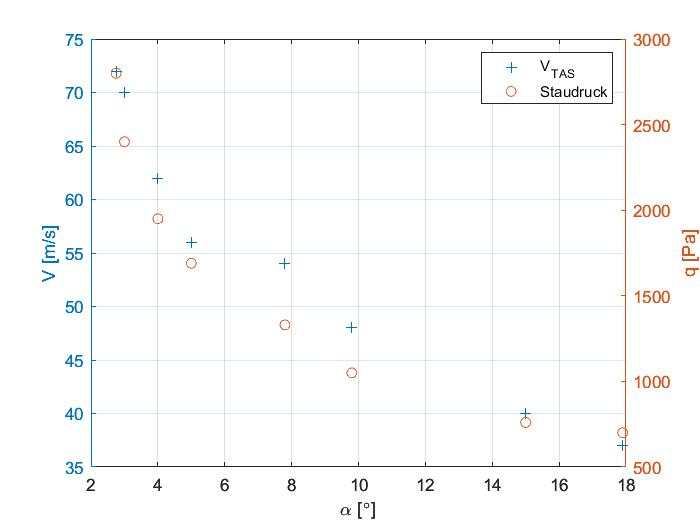
\includegraphics[width=0.7\textwidth]{./Bilder/V_q_alpha.jpg}
	\caption{$V$ und $q$ über $\alpha$ der DO-28}
	\label{fig:V_q_alpha_DO28}
\end{figure}
\chapter{Interpretation der Ergebnisse (NH)}

\section{Höhenruder Trimmkurve}

Im Flugversuch der DO-28 konnten der Anstellwinkel $\alpha$, sowie der Trimmwinkel $\eta$ aufgezeichnet werden. Zur Darstellung sind, nach Selektion der 8 Flugabschnitte, die Werte von $\alpha$ aufgrund der Trimmung $\eta$ aufgetragen. Dabei ist in dem Graph \ref{fig:alpha_eta_DO28} gut zu erkennen, dass die Wertepaare in guter Näherung in einer Flucht liegen. Zur Veranschaulichung wurde dazu eine Regression geplottet, die diesen ersten Eindruck untermauert.  

Es ergibt sich eine negative Steigung der Regressions-Gerade von $1.4$. Bei der Trimmung von $0 \ ^{\circ}$ ergibt sich aus der Regression ein entstehender Anstellwinkel $\alpha$ von $3.7 \ ^{\circ}$. So folgt daraus, dass bei einer Trimmung von $2.7 \ ^{\circ}$ der Anstellwinkel Null beträgt. Im Vergleich zu der Theorie zeigt sich ein sehr realistischer Verlauf der Trimmkurve, bei der keine nennenswerten Abweichungen der Messpunkte von der Regressions-Geraden auffallen.

\section{Auftriebsbeiwert über Anstellwinkel}

Im Plot \ref{fig:CA_alpha_DO28}, in dem $C_A$ über $\alpha$ aufgeführt ist, kann das identische Verhalten der Messpunkte bilanziert werden, wie bei der Trimmkurve. Die Messpunkte weisen ein linear steigendes Verhalten auf, was mit der Theorie übereinstimmend ist. Dazu ist auch hier eine lineare Regression geplottet, um dies zu stützen. Dabei stellt sich eine Gerade ein, deren Steigung bei $0.0772$ liegt. Dieser Wert stellt gleichzeitig das Derivat $C_{A\alpha}$ bzw. den Auftriebsanstieg dar, der aus der Ableitung des Graphens nach $\alpha$ herrührt. Infolge der Regression kann der Auftriebsbeiwert bei einem Anstellwinkel von $0 \ ^{\circ}$ als $C_{A0}$ sowie der Nullauftriebswinkel $\alpha_0$ mit $0.22$ bzw. $-2.89$ bestimmt werden.

Der Graph spiegelt somit den allgemeingültigen Zusammenhang zwischen Anstellwinkel und Auftriebsbeiwert wieder. Dabei hat $\alpha$ per Definition und nach Abgleich mit dem Graphen einen Haupteinfluss auf den Auftriebsbeiwert. So stellt sich für kleine Anstellwinkel wie erhofft ein linearer Verlauf ein \cite{Skript}.

\section{Lilienthal-Polare}

\subsection{DO-128}

Im Graphen \ref{fig:CA_CW_DO128} sind  Auftriebsbeiwerte $C_A$ über Widerstandsbeiwerte $C_W$ der DO-128 geplottet. Neben diesen Messwerten ist eine quadratische Polare berechnet worden, die die Flugzeugpolare darstellt. Deren Faktoren sind in der angefügten Legende ablesbar. \\ Die Polare stellt dabei einen, im Vergleich zur Theorie, übereinstimmenden Graphen dar \cite{Kurzskript}. Dieser generiert für kleine $C_A$ eine zunächst seht steile Steigung, die mit steigendem $C_A$ quadratisch abnimmt. 

Mittels des Schnittpunktes dieser Regression kann der Nullwiderstand $C_{W0}$ mit einem Wert von 0,05 definiert werden. Damit liegt dieser Kennwert in einem realistischen Bereich für ein Flugzeug. Neben dieser Kenngröße können mittels der Tangente vom Ursprung an die Regressionsgerade die minimale reziproke Gleitzahl $\epsilon_{min}$, $C_A^*$ und $C_W^*$ bestimmt werden. Nach Ablesen dieser Werte mit $C_A^*=$1,39 und $C_W^*=$0,15 ergibt sich ein $\epsilon_{min}$ von 0,1. Auch diese Werte können dabei als realistisch betrachtet werden. Bei der berechneten minimalen reziproken Gleitzahl stellt sich ein Bahnneigungswinkel von $\gamma=$-6,2$^{\ \circ}$ ein, der ebenfalls realen Werten für $\gamma$ entspricht und über folgende Gleichung definiert ist:

\begin{equation}
\tan\left(\gamma\right)=-\frac{C_W}{C_A}
\end{equation}

Ergänzend dazu können auch der $\textbf{k}$-Faktor, sowie die Oswald-Zahl $e$ mittels folgender Gleichungen definiert werden:

\begin{equation}
C_{W_{i}}=\frac{C_A^2}{\pi \cdot \Lambda}\cdot \textbf{k}=k*C_A^2, \\ \mathrm{mit} \ \Lambda=8,34 
\label{eq:C_W_i}
\end{equation}
und
\begin{equation}
e=\frac{1}{\textbf{k}}
\end{equation}

Dabei stellt $k$ in Gleichung \ref{eq:C_W_i} den Vorfaktor des Polynoms 2. Grades der quadratischen Regression dar, der in unserem Fall 0,0258 beträgt. Dies stellt allerdings nur eine Näherung dar, da die Regression im Plot \ref{fig:CA_CW_DO128} auch ein lineares Polynom enthält. Nach Berechnung der Gleichungen ergibt sich für $\textbf{k}$ ein Wert von 0,676 und für $e$ ein Wert von 1,5. 
Laut Definition ist jedoch der $\textbf{k}$-Faktor $>1$ und der Oswald-Faktor stets größer als $1$. \\
Diese Unstimmigkeit ist mit hoher Wahrscheinlichkeit auf die quadratische Regression und die damit verbundene unpassende Steigung (hier: 0,0258) zurückzuführen.

\subsection{DO-28}

Bei der Flugzeugpolaren der DO-28 zeigt sich ein sehr ähnlicher Verlauf, wie bei der DO-128. Zu erkennen ist jedoch zunächst, dass die Messpunkte teilweise weit von der erstellen Regressionslinie entfernt sind. Dies sorgt vermutlich auch für den eher bauchigen Verlauf der quadratischen Polaren. Somit ist ein $C_{W0}$ zu verzeichnen, welches mit 0,068 verhältnismäßig groß ist. 

Mittels der Tangente ergibt sich für die minimale reziproke Gleitzahl $\epsilon_{min}$, aus $C_A^*=$1,05 und $C_W^*=$0,092, der Wert 0,09. Auch dieser Wert liegt in einer realistischen Größenordnung für diesen Kennwert.

Der zugehörige Bahnneigungswinkel $\gamma$ hat dabei den Wert -5$^{\ \circ}$ und liegt somit auch im üblichen Bereich. 

Mittels der Regressionsformel kann ebenfalls der $\textbf{k}$-Faktor bestimmt werden, der in diesem Fall bei 1,6 liegt und somit größer als 1 ist (wie per Definition vorgegeben). Der zugehörige Oswald-Faktor $e$ ergibt sich im Anschluss zu 0,6. 

\section{Widerstand über Fluggeschwindigkeit}

\subsection{DO-128}

Im Graphen \ref{fig:W_V_DO128} ist der Widerstand $W$ über die wahre Fluggeschwindigkeit $V_{TAS}$ aufgetragen. Die ermittelten Messpunkte sind darin über eine Linie miteinander verbunden. Eine eindeutig steigende Tendenz des Widerstandes ist mit steigender Fluggeschwindigkeit $V$ zu verzeichnen. Dies bildet den realen bzw. theoretischen Zusammenhang dieser beiden Größen korrekt ab. Dabei steigt der Widerstand in quadratischer Form mit der Fluggeschwindigkeit.

Zur Veranschaulichung der \grqq{optimalen}\grqq{ } Bedingungen bzw. Fluggeschwindigkeit, ist diese mittels Gleichung \ref{eq:V_opt} berechnet worden und in dem Graphen markiert. Dabei ergibt sich für $V_{opt}$ ein Wert von 42,21 \SI{}{\meter\per\second}.

Mittels Gleichung \ref{eq:W_min} wurde ebenfalls der minimale Widerstand berechnet, der mit einem Wert von 2923,28 \SI{}{\newton} nicht im Diagramm eingezeichnet ist. Angesichts des Verlaufs des Graphen stellt dieser Wert ein realistisches Ergebnis für diesen Kennwert dar.

\subsection{DO-28}

Bei dem Verlauf von $W$ über $V$ der DO-28 stellt sich ein etwas anderer Plot dar. Zu erkennen ist, dass die Messpunkte sehr durcheinander und in vertikaler Richtung sehr variabel auftreten. Trotzdem lässt sich tendenziell ein quadratisch ansteigender Verlauf aus dem Plot ableiten. Aufgrund der hohen Variation ist jedoch auf eine Messpunktverbindung verzichtet worden.

Auch hier ist $V_{opt}$ sowie $W_{min}$ mittels Gleichung \ref{eq:V_opt} und \ref{eq:W_min} bestimmt worden. Dabei ergab sich für die optimale Fluggeschwindigkeit, die bei der minimalen reziproken Gleitzahl erreicht wird, der Wert 44,92 \SI{}{\meter\per\second}. \\ Der minimale Widerstand ergab laut Berechnung ein Wert von 4678 \SI{}{\newton}. Dieser liegt jedoch deutlich höher als schon gemessene Widerstandswerte, die im Plot zu erkennen sind. Aufgrund dieser Tatsache ist $W_{min}$ nicht im Plot aufgeführt. \\
Ein entscheidender Grund für diese Abweichung ist mit hoher Wahrscheinlichkeit die schon erwähnte Flugzeugpolare, die aufgrund der Messpunkte ein bauchigen Verlauf zeigt. Dadurch steigt $C_W$ für ein kleiner werdendes $C_A$ ab ca. $C_A=$0,35, bis $C_{W0}$ an.

\section{Staudruck über Anstellwinkel}

Im Graphen \ref{fig:V_q_alpha_DO28} ist der Staudruck $q$ über $\alpha$ abgebildet. Dabei ist gut zu erkennen, dass mit sinkendem Anstellwinkel der Staudruck näherungsweise quadratisch steigt. \\
Ein Grund für dieses Phänomen ist, dass ein steigender Anstellwinkel eine Verlangsamung des Flugzeugs bzw. der Anströmgeschwindigkeit zur Folge hat. Ein weiterer weitaus unbedeutenderer Einflussfaktor ist die nicht frontale Anströmung auf das Pitotrohr infolge eines großen Anstellwinkels, wodurch der angezeigte Staudruck sinkt.

\section{Fluggeschwindigkeit über Anstellwinkel}

Im selben Graphen des Staudrucks ist auch die wahre Fluggeschwindigkeit $V_{TAS}$ über den Anstellwinkel $\alpha$ abgebildet. Dabei ist schnell zu erkennen, dass die Messpunkte der Fluggeschwindigkeit mit geringen Abweichungen mit den Messpunkten des Staudrucks korrelieren. \\
Der Grund für dieses Phänomen ist der formelmäßige Zusammenhang bzw. die Tatsache, dass die angezeigte Fluggeschwindigkeit $V_{IAS}$ aus dem Staudruck $q$ berechnet wird. Dabei ergeben sich im Plot \ref{fig:V_q_alpha_DO28} lediglich kleine Abweichungen, da die angezeigte Fluggeschwindigkeit noch über die Dichte $\rho$ der jeweiligen Höhe bereinigt wird.

\section{Diskussion des Gesamtversuches}

Der Versuch bzw. die Ermittlung der Kenngrößen und Messdaten haben im Allgemeinen zufriedenstellende Ergebnisse und Graphen ergeben. Allerdings sind in manchen Berechnungen und Graphen ein paar wenige Unstimmigkeiten aufgetreten, die mehrere Gründe haben.\\
Zum Einen kommt es infolge der Vielzahl an Rundungen, Ablesefehlern und Abschätzungen einiger Größen zu Abweichungen, die bei weiterer Verrechnung zu unrealistischen Ergebnissen führen können. \ Zum Anderen führen die Regressionen, die zur Bestimmung von Kenngrößen genutzt werden, zu unrealistischen Werten, insbesondere, wenn diese Regressionen bei Messwerten angewendet werden, die starke Ausreißer beinhalten.

Insgesamt konnte durch diesen Versuch jedoch eine realistische Abbildung bzw. Berechnung der Kenngrößen durchgeführt werden.
\chapter{Interpretation der Ergebnisse (FM)}

In diesem Kapitel sollen die gemessen Werte der beiden Flüge, die im vorherigen Abschnitt aufgetragen wurden, zu interpretieren und die Zusammenhänge zu erklären. 

\section{Höhenruder Trimmkurve}
Die Werte für den Anstellwinkel $\alpha$ und den Trimmwinkel $\eta$ konnten direkt aus den jeweiligen Bereichen der Flugschriebe der DO 28 abgelesen werden. Dazu wurde der Verlauf der Kurve bestmöglich gemittelt. Das Auftragen der erhaltenen Werte lässt einen linearen Zusammenhang vermuten. Die Regressionsgerade mit der Formel $\alpha = -1,4043 \cdot \eta + 3,7239$ bestätigt diesen Verdacht. Es gibt nur sehr geringe Abweichung der Messpunkte von der Geraden. Ein stärkerer Ruderausschlag resultiert also in einer proportionalen Vergrößerung des Anstellwinkels um den Faktor $- 1,4043$.
Demnach wird ein Anstellwinkel von $\alpha = 0^{\circ}$ bei einem Trimmwinkel von $\eta = 2,7^{\circ}$ erreicht. Ein Trimmwinkel von $\eta = 0^{\circ}$ resultiert in einem Anstellwinkel von $\alpha = 3,7239^{\circ}$.

\section{Auftriebsbeiwert über Anstellwinkel}
Der Wert des Anstellwinkels $\alpha$ kann aus den entsprechenden Bereichen des Flugschriebs der DO 28 gemittelt abgelesen werden. Der Auftriebsbeiwert $C_A$ wird durch das in Kapitel \ref{sec:CA} beschriebene Vorgehen bestimmt. 
Das Auftragen der erhaltenen Werte lässt ein linearen Zusammenhang zwischen Anstellwinkel und Auftriebsbeiwert vermuten. Dieses Verhalten entspricht der Theorie. Erst in Bereichen nahe des Strömungsabrisses knickt die gerade nach unten ab \citep{Skript}. In unseren Messwerten ist dieses Verhalten nicht zu erkennen, da der Flugversuch nicht an bis an diese kritischen Bereiche geführt wurde.

Die durchgeführte lineare Regression hat den formelmäßigen Zusammenhang $C_A = 0,0772 \cdot \alpha + 0,2234$. Der Auftriebsbeiwert steigt also bei größer werdendem Anstellwinkel proportional um den Faktor $0,0772$. Dieser Faktor wird auch Auftriebsanstieg oder Derivativ $C_{A \alpha}$ genannt. Per Definition ist er die Ableitung des Auftriebsanstiegs nach dem Anstellwinkel $C_{A \alpha} = \frac{\mathrm{d} C_A}{\mathrm{d} \alpha}$, was bei einer linearen Funktion der Steigung entspricht. 

Bei einem Anstellwinkel von $\alpha = 0^{\circ}$ erhalten wir laut der Regression einen Auftriebsbeiwert von $C_{A0} = 0,2234$. Es entsteht also immer noch Auftrieb durch das Flügelprofil. 
Ein Auftriebsbeiwert von $C_{A0} = 0$ wird erst bei dem Nullauftriebswinkel von $\alpha_0 = -2,894^{\circ}$ erreicht.

\section{Lilienthal-Polare}
Die Lilienthal-Polare wurde sowohl für den Flugversuch der DO 28 als auch für den der DO 128 bestimmt. Sie entsteht durch auftragend des Auftriebsbeiwertes $C_A$ über den Widerstandsbeiwert $C_W$. 
Aus der Theorie erwarten wir einen quadratischen Zusammenhang der Form:

\begin{equation}
C_W = C_{W0} (+ j \cdot C_A) + k \cdot C_{A}^2
\end{equation}

Der Term $k \cdot C_{A}^2$ entspricht dabei dem induzierten Widerstand $C_{W_i}$. Durch gleichsetzten dieses Zusammenhangs mit der Formel für den induzierten Widerstand entsteht eine Möglichkeit den k-Faktor und die Oswald-Zahl $e$ zu bestimmen:

\begin{equation}
C_{W_{i}}=\frac{C_A^2}{\pi \cdot \Lambda}\cdot \textbf{k}=k*C_A^2, \\ \mathrm{mit} \ \Lambda=8,34 
\label{eq:C_W_i}
\end{equation}

\begin{equation}
k = \frac{\textbf{k}}{\pi \cdot \Lambda}
\end{equation}

\textbf{DO 128}

Mit diesen Zusammenhängen lässt sich ein k-Faktor von $0,676$ bestimmen, was einer Oswald-Zahl von $e = 1,5$ entspricht. Diese Kennwerte entsprechen jedoch nicht der Definition, da der k-Faktor stets größer Null ist und die Oswald-Zahl stets kleiner als Null. Die Abweichung der Werte von der Theorie ist wahrscheinlich mit der ungenauen Regression zu erklären.

Anhand des Schnittpunktes der Regression mit der x-Achse, lässt sich der Nullwiderstand $C_{W0} = 0.5$. Dieser Wert liegt durchaus im realistischen Bereich. Weitere Kennwerte lassen sich durch anlegen einer Tangente an die Regression bestimmen, die durch den Ursprung führt. Der Berührungspunkt ist der Punkt des besten Gleitens und es lassen sich sowohl $C_W^* = 0,15$ als auch $C_A^* = 1,39$ ablesen. Aus diesen beiden Werten lassen sich wiederum eine minimale reziproke Gleitzahl von $\epsilon_{min} = 0,1$ und nach Formel \ref{Bahn} der entsprechende Bahnneigungswinkel zu $\gamma=-6,2^{\ \circ}$ bestimmen. Beide Werte sind durchaus im realistischen Rahmen.

\begin{equation}
\tan\left(\gamma\right)=-\frac{C_W}{C_A}
\label{Bahn}
\end{equation}

\textbf{DO 28}

Auffällig bei der Lilienthal-Polaren der DO 28 ist, dass die Messwerte zum Teil deutlich weiter von der Regressionskurve entfernt sind. Dennoch lassen sich die selben Kennwerte bestimmen wie im vorherigen Abschnitt. 
Der k-Faktor, der sich aus der Regressionsformel bestimmen lässt beträgt in diesem Fall $1.6$ und entspricht damit der Definition, dass er größer als 1 ist. Der entsprechende Oswald-Faktor beträgt $e = 0,6$, was ebenfalls der Definition $e<1$ entspricht. 
Der Nullwiderstand, der sich aus dem x-Achsen Schnittpunkt bestimmen lässt ist mit einem Wert von $C_{W0} = 0,068$ etwas zu groß, was eventuell auf die relativ großen Abweichungen zwischen Messwerten und Regression zurückzuführen ist.
Mit der Tangente lassen sich die Kennwerte des besten Gleitens zu $C_A^* = 1,05$ und $C_W^* = 0,092$ bestimmen, was einer minimalen reziproken Gleitzahl von $\epsilon_{min} = 0,09$ entspricht. Daraus lässt sich der Bahnneigungswinkel von $\gamma = -5^{\ \circ}$. Alle diese Werte liegen in einem Bereich, der durchaus üblich für entsprechende Flugzeuge ist.


\section{Widerstand über Fluggeschwindigkeit}
Laut der Theorie setzt sich der Widerstand zum einen aus dem Nullwiderstand $W_0$ und zum anderen aus dem Auftriebswiderstand $W_A$. Beide Komponenten zeigen einen exponentiellen Verlauf über die Fluggeschwindigkeit, jedoch hat die Funktion des Nullwiderstands einen positives Exponenten und steigt, während die Funktion des Auftriebswiderstands einen negativen Exponenten besitzt und somit mit steigender Geschwindigkeit sinkt. Die Überlagerung beider Funktion weißt also einen Tiefpunkt auf, bevor sie ins unendliche ansteigt. Per Definition tritt dieser Tiefpunkt bei der Geschwindigkeit von $V_{opt}$. Da sich $V_{opt}$ beim besten Gleiten einstellt, lässt sich $V_{opt}$ aus den Kennwerten des besten Gleitens nach Formel \ref{eq:V_opt} bestimmen. Für die DO 128 ergibt sich ein Wert von $V_{opt} = 42,21 \frac{m}{s}$. Dieser Wert ist auch im Graphen eingezeichnet, es wird jedoch relativ deutlich, dass dieser Wert nur schlecht zu dem Verlauf passt. Der Tiefpunkt des Graphen scheint erst bei wesentlich geringeren Geschwindigkeiten aufzutreten. Wahrscheinlich stammt dieser Fehler aus der Regression der Lilienthal-Polaren und damit aus Abweichungen bei der Bestimmung von $C_A^*$ und $C_W^*$. Zusätzlich lässt sich der minimale Widerstand nach Gleichung \ref{eq:W_min} berechnen, der theoretisch im Tiefpunkt des Graphen zu finden wäre. Auf diese Weise kann ein Wert von $W_{min} = 2923,28$ N bestimmen. Wenn man den Verlauf der Messwerte im Diagramm der DO 128 \ref{fig:W_V_DO128} betrachtet, scheint dieser relativ gut zu den Werten zu passen.

Die Messwerte der DO 28 sehen allerdings noch schlechter aus. Der erwartete Verlauf lässt sich nur schwer erahnen. Rechnerisch lässt sich $V_{opt} = 44,92 \frac{m}{s}$ zwar bestimmen und in das Diagramm einzeichnen, auch hier ist aber auffällig, dass dieser Wert nur schlecht zu dem Verlauf der Messwerte passt. Nach Gleichung \ref{eq:W_min} lässt sich für die DO 28 ein minimaler Widerstand von $W_{min} = 4678$ N bestimmen. Da wir in der Messreihe allerdings niedrigere Widerstände aufgenommen haben, passt der rechnerisch bestimmte Wert nicht zu erstellten Graphen. Aus diesem Grund haben wir uns dafür entschieden $W_{min}$ nicht in das Diagramm aufzunehmen. Auch in diesem Fall ist die Ursache des Problems sehr wahrscheinlich eine ungünstige quadratische Regression der Lilienthal-Polaren. Der Nullwiderstand $C_{W0}$ ist in der Realität wahrscheinlich deutlich kleiner als der von uns abgelesene Wert, was dazu führt, dass ein zu großer minimaler Widerstand berechnet wurde.

\section{Staudruck und Fluggeschwindigkeit über Anstellwinkel}
In Diagramm \ref{fig:V_q_alpha_DO28} sind sowohl der Staudruck $q$, als auch die wahre Fluggeschwindigkeit $V_{TAS}$ Anstellwinkel $\alpha$ aufgetragen. Es wird deutlich, dass beide Werte einen qualitativ sehr ähnlichen Verlauf zeigen. Das ist in sofern logisch, dass die wahre Fluggeschwindigkeit sich aus dem Staudruck und der Luftdichte berechnen lässt.

\begin{equation}
V_{TAS}= \sqrt{\frac{2 \cdot q}{\rho}}
\end{equation}

Da sich die Luftdichte über die Flugabschnitte nur in geringem Maße ändert, erhalten wir eine nahezu direkte Abhängigkeit der beiden Messreihen, was den ähnlichen verlauf erklärt. 

Mit steigendem Anstellwinkel $\alpha$ sinken sowohl die Fluggeschwindigkeit, als auch der Staudruck. Das ist damit zu erklären, dass ein höherer Anstellwinkel den Auftriebsbeiwert $C_A$ steigert. Je höher der Auftriebsbeiwert, desto geringer ist die Geschwindigkeit, die zum Gleiten benötigt wird. 

\section{Diskussion des Gesamtversuches}
Insgesamt konnten durch den Versuch überwiegend zufriedenstellende Ergebnisse erzielt werden. Der Großteil der Messdaten und ermittelten Kennwerte entsprechen der theoretischen Grundlage. Es gibt allerdings auch ein paar Punkte, in denen die Messdaten sich zum Teil deutlich von den Erwartungen unterscheiden. Ursache für diese Abweichungen ist vor allem das Auswerten der Flugschriebe per Hand. Dabei wurde häufig nur bestmöglich abgelesen und gerundet, wobei stets kleinere Fehler auftreten können. Diese Fehler werden größer, wenn mit ihnen im weiteren Verlauf gerechnet wird und vor allem, wenn Regressionen durch diese unter Umständen ungenauen Messwerte gelegt werden. Vor allem Ausreißer fallen bei einem kleinen Datenumfang stark ins Gewicht. Auf diese Weise ist es möglich, dass unrealistische Ergebnisse entstehen, die nicht mit der Theorie vereinbar sind. In unseren Versuchen stellt das allerdings die Ausnahme dar.
\chapter{Interpretation der Ergebnisse (TG)}

Nachfolgend sollen die Daten, welche jeweils in den Flugversuchen mit den Flugzeugen DO-128 und DO-28 aufgenommen und in den Diagrammen in Abschnitt \ref{c:Ergebnisse} dargestellt worden sind, interpretiert werden. Die Messpunkte in den Graphen der DO-128 resultieren aus den vier Abschnitten, welche erflogen wurden. Für die Messschriebe der Flugversuche mit der DO-28 wurden für alle Versuchsschriebe identisch acht Flugabschnitte definiert (siehe Anhang). Alle Daten wurden anhand dieser ausgewertet. Bestimmend für die Flugabschnitte waren dabei zwei Aspekte: a) Höhe $h$ abnehmend (Sinkflug)  b) Bereich annähernd konstanter Geschwindigkeit $v_{TAS}$. 


\section{Höhenruder Trimmkurve}
Aus den Versuchsschrieben der Kanäle 4 und 5 der DO-28 wurden die Werte der Anstellwinkel $\alpha$ und der Trimmwinkel $\eta$ für die acht Abschnitte jeweils gemittelt abgelesen. In dem Diagramm \ref{fig:alpha_eta_DO28} sind die Werte für $\alpha$ über $\eta$ aufgetragen. Durch die Punkte wurde mittels linearer Regression eine Gerade gelegt. Die angewendete lineare Regressionsformel lautet $\alpha = -1,4043 \cdot \eta + 3,7239$. 

Bei einem Anstellwinkel von $\alpha = 0^{\circ}$ muss ein Trimmwinkel von $\eta = 2,7^{\circ}$ eingestellt werden. Bei einem Trimmwinkel von $\eta = 0^{\circ}$ nimmt der Anstellwinkel den Wert $\alpha = 3,7239^{\circ}$ an. 

An dem Graphen \ref{fig:alpha_eta_DO28} erkennt man sehr gut, dass der Anstellwinkel $\alpha$ und der Trimmwinkel $\eta$ direkt linear voneinander abhängen. Mit stärkeren Ausschlägen des Ruders in negative Richtung steigt ebenfalls der Anstellwinkel proportional um den Faktor $- 1,4043$ an.

Vergleichend mit den Theoriewerten ist dies zu erwartendes Verhalten. Es gibt keine nennenswerten Abweichungen der Messpunkte von der Regressionsgerade. 


\section{Auftriebsbeiwert über Anstellwinkel}
Der Anstellwinkel $\alpha$ wurde in den Versuchsschrieben der DO-28 auf Kanal 4 aufgezeichnet und kann für die acht Abschnitte abgelesen werden.

Der Auftriebsbeiwert $C_A$ kann gemäß Abschnitt \ref{sec:CA} aus der Formel \ref{eq:CA} bestimmt werden. Für die Berechnung gehen die Flügelfläche $S$, die Masse $m$, die Sinkgeschwindigkeit $w_{r_{real}}$, die Fluggeschwindigkeit $v_{TAS}$ und die Luftdichte $\rho_{real}$ ein. Diese Werte können den Messchrieben entnommen werden.

Der Auftriebsbeiwert $C_A$ wurde über den Anstellwinkel $\alpha$ in Diagramm \ref{fig:CA_alpha_DO28} aufgetragen. Dabei stellt sich ein linearer Zusammenhang ein, weswegen erneut eine lineare Regression mit der Geradengleichung $C_A = 0,0772 \cdot \alpha + 0,2234$ angesetzt wurde. Diese Regression genügt für kleine Anstellwinkel der Gleichung 

\begin{equation}
C_A = C_{A \alpha} (\alpha - \alpha_0)
\end{equation}

Es ist erkennbar, dass bei steigendem  Anstellwinkel $\alpha$ auch der Auftriebsbeiwert $C_A$ um den Faktor $C_{A \alpha} = 0,0772$ ansteigt.  
Der Faktor $C_{A \alpha}$ heißt Auftriebsanstieg oder Derivativ und ist per Definition die Ableitung des Auftriebsbeiwerts nach dem Anstellwinkel $C_{A \alpha} = \frac{\mathrm{d} C_A}{\mathrm{d} \alpha}$. 

Bei einem Nullanstellwinkel $\alpha = 0^{\circ}$ nimmt der Auftriebsbeiwert den Wert $C_{A0} = 0,2234$ an. Dass heißt, auch wenn der Flügel nicht angestellt ist, erzeugt er aufgrund seiner Profilgeometrie einen Auftrieb. Damit das Profil keinen Auftrieb mehr erzeugt, muss es um den Nullauftriebswinkel $\alpha_0 = -2,894^{\circ}$ angestellt werden.

Bei größeren Anstellwinkeln würde die Kurve aufgrund von Strömungsabriss am Profil ab $C_{A_{max}}$ nichtlinear stark fallen.

Dieser Graph entspricht der Theorie für kleine Anstellwinkel. Die aufgezeichneten Werte genügen dem erwarteten linearen Verlauf.


\section{Lilienthal-Polare}
Sowohl für die Flugversuche der DO-128 als auch die der DO-28 wurde in den Diagrammen \ref{fig:CA_CW_DO128} und \ref{fig:CA_CW_DO28} der Auftriebsbeiwert $C_A$ über den Widerstandsbeiwert $C_W$ aufgetragen. Weiterhin wurde mittels Polynomansatz zweiten Grades eine Regression durchgeführt und so die quadratische Polare nach folgendem Ansatz bestimmt:

\begin{equation}
C_W = C_{W0} (+ j \cdot C_A) + k \cdot C_{A}^2
\end{equation}

Die Werte der Faktoren j, k und der Wert $C_W0$ für das jeweilige Flugzeug sind in der Legende der Diagramme vermerkt. Diese Polare wird als Lilienthal-Polare bezeichnet. Aus diesem Diagramm kann für verschiedene Bahnwinkel $\gamma = \epsilon = - \frac{C_W}{C_A}$, wobei $\epsilon$ als reziproke Gleitzahl bezeichnet wird, die vorherrschenden Beiwerte ermittelt werden. 

Weiterhin wurden in die beiden Diagramme jeweils eine Tangente vom Ursprung gelegt. Der Winkel dieser Tangente zur x-Achse ist die minimale reziproke Gleitzahl $\epsilon_{min}$. Am Berührungspunkt der Tangente mit der Lilienthal-Polare können die Beiwerte für das beste Gleiten abgelesen werden. Diese sind für die DO-128 $C_{A_{128}}^* = 1,39$ sowie $C_{W_{128}}^* = 0,105$ und für die DO-28 $C_{A_{28}}^* = 1,045$ sowie $C_{W_{28}}^* = 0,0916$. In diesem Flugzustand, nimmt die reziproke Gleitzahl $\epsilon$ den kleinsten Wert an und das Flugzeug gleitet am weitesten. Dies ist jedoch der Zustand, bei dem die Sinkgeschwindigkeit am geringsten ist. Das wird als Fahrt mit minimaler aerodynamischer Verlustleistung bezeichnet und ist bei $C_W = 4 \cdot C_{W0}$ und $C_{A_{wg,min}} = \sqrt{3} \cdot C_A^*$. Das beste Gleiten findet jedoch bereits bei $C_W^* = 2 \cdot C_{W0}$ statt. Der Wert $C_{W0}$ wurde mittels Regression für die DO-128 zu $C_{W0_{128}} = 0,05$ und für die DO-28 zu $C_{W0_{28}} = 0,0684$ bestimmt. 


Wie in dem Diagramm \ref{fig:CA_CW_DO128} zu erkennen ist, passt die Regression für die quadratische Polare der DO-128 sehr gut zu den Daten der ermittelten Beiwerte. In Diagramm \ref{fig:CA_CW_DO28} zeigt sich jedoch, dass die Regression der DO-28 nur unzureichend für die Daten der ermittelten Beiwerte passt.


\section{Widerstand über Fluggeschwindigkeit}
Für die DO-128 wurde der Widerstand $W$ über die Fluggeschwindigkeit $V_{TAS}$ in Diagramm \ref{fig:W_V_DO128} aufgetragen. Es ist zu sehen, dass bei steigender Fluggeschwindigkeit auch der Widerstand infolge von Reibungsverlusten steigt. Der Widerstand ist dabei eine Überlagerung des Nullwiderstandes $W_0$, welcher Widerstand durch Reibung und einer exponentiellen Funktion mit positiven Exponenten folgt und des Auftriebswiderstandes $W_A$, welcher infolge des Widerstandes induziert wird und einer exponentiellen Funktion mit negativen Exponenten folgt. Dieser Argumentation folgen, nimmt der Widerstand einen Minimalwert an, welcher definitionsgemäß bei $V_{opt}$ liegt. Dieser minimale Widerstand stellt sich bei der minimalen reziproken Gleitzahl $\epsilon_{min}$ ein, welche bereits in den Diagrammen der Lilienthal-Polare bestimmt wurde. Aus den Beiwerten der optimalen Gleitzahl kann nach Gleichung \ref{eq:V_opt} die optimale Fluggeschwindigkeit für die DO-128 zu $V_{opt_{128}} = 42,21 \frac{m}{s}$ und nach Gleichung \ref{eq:W_min} der minimale Widerstand zu $W_{min_{128}} = 2636,3 N$ bestimmt werden. Wie aus den Graph \ref{fig:W_V_DO128} jedoch ersichtlich ist, passen diese beiden Werte nicht zueinander. Grund hierfür könnte eine Abweichung des Punktes des besten Gleitens und damit der Beiwerte durch die angesetzte Regression der quadratischen Polare sein, wobei die Masse des Flugzeuges für den Punkt des besten Gleitens gemittelt werden musste. 


Gleiches wurde mit den Daten der DO-28 in Diagramm \ref{fig:W_V_DO28} getan. Es ist zu sehen, dass sich daraus nur wage Rückschlüsse auf den Verlauf des Widerstandes $W$ über der Fluggeschwindigkeit $V_{TAS}$ ziehen lassen. Nach der Theorie, müssten die Punkte einen ähnlichen Verlauf wie in Diagramm \ref{fig:W_V_DO128} annehmen. Auch hier kann aus den Beiwerten der optimalen Gleitzahl kann nach Gleichung \ref{eq:V_opt} die optimale Fluggeschwindigkeit für die DO-28 zu $V_{opt_{28}} = 44,92 \frac{m}{s}$ und nach Gleichung \ref{eq:W_min} der minimale Widerstand zu $W_{min_{28}} = 4678 N$ bestimmt werden. Auch hier passen die Werte nicht gut aufeinander. Dies lässt schlussfolgern, dass auch hier die angesetzte Regression der quadratischen Polare in dem Diagramm \ref{fig:CA_CW_DO28} ungenau ist, womit der Punkt des besten Gleitens und dessen Beiwerte nur ungenau ermittelt werden können.

\section{Staudruck und Fluggeschwindigkeit über Anstellwinkel}
Der Staudruck $q$, die Fluggeschwindigkeit $V_{TAS}$ und der Anstellwinkel $\alpha$ wurden in den Versuchsschrieben der DO-28 auf den Kanälen 2 und 4 aufgezeichnet und für die acht Bereiche ermittelt. In dem Diagramm \ref{fig:V_q_alpha_DO28} wurde der Staudruck $q$ in \SI{}{\pascal} als rote Kreise und die Fluggeschwindigkeit $V_{TAS}$ in \SI{}{\meter \per \second} als blaue Kreuze über den Anstellwinkel $\alpha$ aufgetragen.

$V_{TAS}$ und $q$ zeigen einen ähnlichen Verlauf. Dies ist auch logisch, da der Staudruck von der Fluggeschwindigkeit abhängt und die Fluggeschwindigkeit daher aus dem Staudruck mit folgender Gleichung berechnet werden kann:

\begin{equation}
V_{TAS} = \sqrt{2 \cdot \frac{q}{\rho}}
\end{equation}

Je steiler der Anstellwinkel $\alpha$ ist, desto langsamer fliegt das Flugzeug, $V_{TAS}$ sinkt und desto geringer ist der Staudruck $q$. Dieses Verhalten kann man sehr gut an dem Graphen \ref{fig:V_q_alpha_DO28} erkennen. 

\chapter{Interpretation der Ergebnisse (AG)}


\section{Höhenruder Trimmkurve}
Es wurde der Anstellwinkel Alpha über dem Höhenruder Trimmwinkel aufgetragen. Danach wurde eine lineare Regression vorgenommen, die Regressionsgerade hat die Gleichung $\alpha= -1,4043*\eta + 3,7329$. Die aufgetragenen Werte liegen sehr nahe an der Geraden. Ein negatives eta entspricht einem Ruderausschlag nach oben, dann wird am Heck Abtrieb erzeugt und die Flugzeugnase hebt sich. Der Verlauf der Geraden ist dabei realistisch, je größer der Ausschlag am Ruder wird, desto stärker hebt sich die Flugzeugnase, dabei gibt es einen linearen Zusammenhang.
 
\section{Auftriebsbeiwert über Anstellwinkel}
Hier wurde der Auftriebsbeiwert $C_A$ über dem Anstellwinkel $\alpha$ aufgetragen. Danach wurde mit einer linearen Regression eine Regressionsgerade bestimmt, dabei passt die Gerade sehr gut denn alle aufgetragenen Punkte liegen nahe an der Geraden. Die Gleichung der Regressionsgeraden lautet: $C_A=0,0772 \alpha +0,2234$. Die Werte stimmen mit der Theorie überein, je größer der Anstellwinkel wird, desto größer wird auch der Auftrieb des Tragflügels. Bei noch steileren Anstellwinkeln kommt man zu dem Bereich wo die Strömung nicht mehr sauber um den Flügel strömen kann, es kommt zum Strömungsabriss. Die Gerade würde dann schnell nach unten abknicken, dieser Bereich ist im Graphen nicht eingezeichnet. Da es sich um einen profilierten Flügel handelt wird bei einem Anstellwinkel von null Grad immer noch Auftrieb erzeugt, dann liegt der Auftriebsbeiwert bei $C_{A0}$ bei 0,2234. Der Nullauftriebswinkel bei dem der Flügel keinen Auftrieb mehr erzeugt liegt bei $\alpha _0 = -2,894^\circ$. $C_{A0}$ und $\alpha_0$ wurde mit Hilfe der Regressionsgeraden bestimmt.

\section{Lilienthal-Polare}
\textbf {Do 128}\\
Für die Lilienthal-Polare wurde der Auftriebsbeiwert $C_A$ über den Widerstandsbeiwert $C_W$ aufgetragen. Für die eingezeichneten Punkte wurde eine quadratische Regression durchgeführt, die Gleichung der Regressionskurve lautet: $C_W= 0,0503+0,0033\ C_A+0,0258\ {C_A}^2$. Die Punkte liegen sehr nahe an der Kurve und stimmen auch gut mit der Theorie überein. Mit steigendem Auftrieb steigt auch der Widerstand des Flugzeugs immer stärker an, bei wenig Auftrieb steigt der Widerstand nur leicht an. Nach der Regression wurde eine Tangente durch den Ursprung gelegt, beim Berührungspunkt von Tangente und Kurve können nun die Werte für optimales Gleiten $C_A^*$ und $C_W^*$ abgelesen werden, dabei ist $C_A^*=1,39$ und $C_W^*=0,105$. Der Nullwiderstandsbeiwert, den das Flugzeug auch ohne Auftrieb hat, kann am X-Achsenschnittpunkt abgelesen werden und beträgt $C_{W0}=0,05$. Weiterhin kann man in dem Diagramm die minimale reziproke Gleitzahl $\epsilon_{min}=0,076$ bestimmen mit $\epsilon_{min}= C_W^* / C_A^*$. Zusätzlich kann dann noch der Bahnneigungswinkel $\gamma=arctan(-\epsilon)=-4,3^\circ$ berechnet werden. 

\textbf {Do 28}\\
Der Aufbau dieses Graphen für den Lilienthal-Polare ist genauso wie bei der Do 128, auch die Werte werden auf die gleiche Art bestimmt. Der eingetragenen Punkte haben diesmal einen großen Abstand zu der quadratischen Polaren, die Werte sind weit verstreut. Besonders zwei Werte bei $C_W=0,07$ und bei $C_W=0,09$ haben eine besonders große Abweichung von der Kurve. Dadurch ergibt sich eine Kurve bei der bei niedrigen Auftriebsbeiwerten unterhalb von $C_A=0,03$ der Widerstandsbeiwert wieder ansteigt. Dieser Verlauf tritt zum Teil auch bei präziser bestimmten Kurven auf. Die Kurvengleichung lautet: $C_W= 0,0678-0,0441\ C_A+0,0642\ {C_A}^2$. Dann werden $C*_A=1,05$ und $C*_W=0,09$ abgelesen, sowie $C_{W0} =0,07$. Dann ist $\epsilon=0,086$ und $\gamma=4,9^\circ$. 
%Mit den Daten für diesen Graphen wurde noch der Widerstandsanstieg $k=1,6216$ mit $C_W=C_{W0}+k*C_A^2$ berechnet. Mit Hilfe der Flügelstreckung der Do128 von $\Lambda=8,04$

\section{Widerstand über Fluggeschwindigkeit}
\textbf {Do 128}\\
Hier wurde der Widerstand des Flugzeugs Do 128 über die Fluggeschwindigkeit in Metern pro Sekunde aufgetragen. Die einzelnen Messpunkte wurden miteinander verbunden, dabei sieht man das bei steigender Geschwindigkeit der Widerstand immer stärker ansteigt. Der berechnete minimale Widerstand $W_{min}=2923,3\ N$ wurde nicht im Diagramm eingezeichnet, dieser liegt außerhalb der gemessen Werte. Die berechnete optimale Geschwindigkeit $V_{opt}=42,21\  ms^{)-1}$ ist gerade die Geschwindigkeit bei dem der Gesamtwiderstand am geringsten ist. Das passt nicht zusammen da $V_{opt}$ nicht bei  $W_{min}$ liegt. Allerdings beträgt der Widerstand bei $V_{opt}$ ungefähr $3050\ N$ und hat damit nur etwa $125\ N$ Abstand zu $W_{min}$. Bei niedrigeren Geschwindigkeiten würde der Widerstand durch den zunehmenden Auftriebswiderstand wieder ansteigen, dieser Bereich ist im Graphen nicht zu sehen.

\textbf {Do 28}\\
Die Werte sind in diesem Diagramm weit verstreut und wurden deshalb auch nicht verbunden, da sich kein sinnvoller Verlauf ergibt. Die optimale Geschwindigkeit beträgt $V_{opt}=44,92\  ms^{)-1}$. Der berechnete minimale Widerstand liegt bei $W_{min}=4678,4\ N$ und damit sogar oberhalb der meisten Messpunkte. Dieser Fehler lässt sich zum Teil durch den zuvor im $C_A C_W$ Diagramm bestimmten großen Wert von $C_{W0}$ erklären, wobei dort schon einige Messwerte starke Abweichungen hatten. Besonders zwei Punkte bei $V=54\ ms^{-1}$ und bei $V=70\ ms^{-1}$ weichen stark von den restlichen Punkten ab. Ohne diese beiden Punkte kann man sich einen Verlauf vorstellen bei dem bei niedrigen Geschwindigkeiten der Widerstand durch den Auftriebswiderstand noch groß ist, dann kommt der Widerstand zu einem Minimum und steigt dann mit zunehmender Geschwindigkeit immer stärker an. Das würde einem theoretischen Verlauf entsprechen.

\section{Staudruck und Fluggeschwindigkeit über Anstellwinkel}
Staudruck und Fluggeschwindigkeit wurden im gleichen Diagramm über dem Anstellwinkel eingezeichnet und haben ungefähr den gleichen Verlauf. Das ist sinnvoll, da die Fluggeschwindigkeit direkt aus dem Staudruck mit $V=\sqrt{(2*q)/\rho}$ berechnet werden kann. Die beiden Wertereihen folgen ungefähr einem quadratischen Verlauf, auch wenn in diesem Fall auf eine Regression verzichtet wurde. Die Werte sind sinnvoll und passen zur Theorie, je steiler der Anstellwinkel des Flugzeugs wird, desto langsamer wird der Flieger.

\section{Diskussion des Gesamtversuches/Fehlerdiskussion (AG)}
Insgesamt wurden bei dem Flugversuch mit der Do 128 Werte gewonnen die bei der Auswertung dem theoretisch erwarteten Verlauf folgen. Fehler wurden hier bei der Messdatenaufnahme besonders durch die ungenauen Ablesemethoden per Hand gemacht. Eine elektronische Messdatenaufzeichnung hätte genauere Werte geliefert.
Bei den gegebenen Messdaten der Do 28 gibt es größere Abweichungen vor der Theorie, obwohl hier die Daten elektronisch aufgezeichnet wurden. Insbesondere beim $C_A C_W$ Diagramm und beim $W V$ Diagramm streuten die Daten sehr weit. Fehler wurden hier beim Ablesen der gedruckten Messwerte auf dem Papier gemacht. Dieser Fehler könnte durch Verwendung der elektronischen Aufzeichnungen vermieden werden. Auch wurden stark oszillierende Messwerte über einen längeren Zeitraum gemittelt wodurch weiter Fehler entstehen.
Bei den Berechnungen wurden die Masse gemittelt so dass dort am Anfang und Ende der Sinkflüge Abweichungen von der tatsächlichen Masse entstehen. Bei der Do 28 wurde der Kraftstoffverbrauch nur über eine lineare Interpolation bestimmt ohne Momentanverbrauch zu berücksichtigen. Zwischenergebnisse wurden gerundet wenn zu viele Nachkommastellen vorhanden waren.
Trotzdem konnte ein guter Einblick in den Umgang mit realen Messdaten gewonnen werden und auch die Vorgehensweise bei einer Auswertung eines praktischen Versuches konnte geübt werden.  Es wurde gezeigt das schon mit wenigen Messdaten die relevanten Kennwerte eines Flugzeuges bestimmt werden können.
\chapter{Interpretation der Ergebnisse (VR)}

\section{Höhenruder Trimmkurve}

Aus den aufgezeichneten Daten im Diagramm \ref{fig:alpha_eta_DO28} lässt sich ein linearer Zusammenhang zwischen dem Anstellwinkel $\alpha$ und dem 
Höhenruderausschlag $\eta$ feststellen. Die entsprechende Regressionsformel lautet $\alpha = -1,4043 \cdot \eta + 3,7239$. Mit steigendem Höhenruderausschlag sinkt der Anstellwinkel. 
Der Anstellwinkel $\alpha$ beschreibt den Winkel zwischen dem Fluggeschwindigkeitsvektor und der Flugzeuglängsachse. Ein positiver Winkel $\alpha$ bedeutet, dass die Flugzeuglängsachse positiv gegenüber dem Fluggeschwindigkeitsvektor gedreht ist \cite{Skript}. 

\begin{figure}[h]
		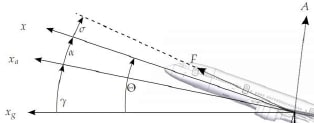
\includegraphics{./Bilder/Anstellwinkel_Definition.jpg}
	\caption{Definition Anstellwinkel}
	\label{alpha_def}
\end{figure}

Der Winkel des Höhenruders $\eta$ beschreibt die Auslenkung des Ruders gegenüber einer Neutrallage. Ein negativer 
Höhenruderausschlag bedeutet eine lokale Absenkung des Auftriebs am Höhenleitwerk, sodass es zum Absinken des Hecks kommt (Nose-up). In die positive Richtung ausgeschlagen steigt der Auftrieb am Höhenleitwerk, sodass sich das Heck hebt (Nose-down). 
Damit decken sich die Messdaten der Do 28 zu Anstellwinkel und Höhenruderausschlag mit der Theorie.




\section{Auftriebsbeiwert über Anstellwinkel}

Der Auftriebsbeiwert $C_A$ steigt linear mit zunehmendem Anstellwinkel $\alpha$. Bei einem Anstellwinkel von $0 \ ^{\circ}$ beträgt der Auftriebsbeiwert $C_{A0}=0,2234$. Der Nullauftriebswinkel $\alpha_{0}$ ist mit $2,894 \ ^{\circ}$ der Winkel, an dem kein Auftrieb mehr erzeugt wird. Der Auftriebsanstieg $C_{A\alpha}$ berechnet sich wie folgt \cite{Skript}:

\begin{equation}
C_{A\alpha}=\frac{dC_A}{\alpha}=0,0772
\end{equation}

	
Bei der Anströmung eines Tragflügels wird die Luft umgelenkt und es entsteht eine Druckdifferenz zwischen Tragflügelober- und Oberseite, was als Voraussetzung für die Entstehung von Auftrieb ist. Der Anstellwinkel des Flügels ist dabei der größte Einflussfaktor für den Auftriebsbeiwert. Für kleine Winkel $\alpha$ mit anliegender Strömung gilt daher der lineare Zusammenhang \cite{Skript}

\begin{equation}
C_A=C_{A\alpha} \left(\alpha - \alpha_0\right)
\end{equation}

Damit stimmen die Messdaten mit der Theorie überein. Jedoch lassen sich keine Aussagen über den maximalen Auftriebsbeiwert treffen, da die aufgenommenen Anstellwinkel im Bereich der anliegenden Strömung liegen und der höchste Auftriebsbeiwert erst kurz vor dem Abreißen der Strömung erreicht wird. 

\section{Lilienthal-Polare}

\textbf{Do 128}

Die für $C_A$ und $C_W$ errechneten Werte werden für die Erstellung der Lilienthalpolare im Diagramm \ref{fig:CA_CW_DO128} gegeneinander aufgetragen und die quadratische Polare lässt sich mit folgendem Ansatz \cite{Skript} bestimmen:

\begin{equation}
C_W = C_{W0} (+ j \cdot C_A) + k \cdot C_{A}^2
\end{equation}

 Daraus ergibt sich für den Nullwiderstand $C_{W0}$ ein Wert von 0,0503, für den Polynomterm erster Ordnung ein Koeffizient $j$ von 0,0033 und für den zweiten Grades ein Koeffizient $k$ von 0,0258. 
Aus der Lillienthal-Polare lässt sich die minimale reziproke Gleitzahl ermitteln, die die Höhendifferenz beim Sinken des Flugzeugs bei einer bestimmten Flugstrecke beschreibt. Zur Ermittlung der minimalen reziproken Gleitzahl wird eine Tangente durch den Ursprung an die entstandene Polare gelegt. Am Schnittpunkt der Tangente mit der Polaren können die zugehörigen Beiwerte $C_A^*=$1,39 und  $C_W^*$=0,105 abgelesen werden, mit denen die reziproke Steigung der Tangente mit

\begin{equation}
\epsilon_{min}=\frac{C_{W}^{\ast}}{C_{A}^{\ast}}=\frac{0,105}{1,39}=0,0755
\end{equation}

berechnet werden kann. Der Gleitwinkel $\gamma$, der die Drehung des Geschwindigkeitsvektor gegenüber der geodätischen Horizontalebene in x-Richtung beschreibt \cite{Skript}, ergibt sich zu

\begin{equation}
\gamma=\arctan \left(-\frac{C^{*}_W}{C^{*}_A} \right)= \arctan \left(-\frac{0,105}{1,39} \right)= -4,32 \ ^{\circ}  
\end{equation}

Aus den bekannten Werten $C_{W0}$ und $C^{*}_A$ lässt sich der Widerstandsanstieg k wie folgt berechnen: 

\begin{equation}
C_{W_{i}}=\frac{C_A^2}{\pi \cdot \Lambda}\cdot \textbf{k}=k*C_A^2, \\ \mathrm{mit} \ \Lambda=8,34 
\end{equation}

\begin{equation}
\textbf{k}= \frac{k}{\pi \cdot \Lambda}=0,676
\end{equation}


Das entspricht einer Oswaldzahl von $e=1,5$. Der Oswaldfaktor ist ein Formeffizienzfaktor, der die Abweichung des Tragflügels vom Optimum bei elliptischer Triebwerksverteilung berücksichtigt. In der Theorie wird an dieser Stelle $e\leq 1$ und $k\geq $ erwartet, was bedeutet, dass die aus der Regression entnommenen Werte falsch sind. Da nur vier verschiedene Flugzustände aufgenommen werden konnten, ist die Regression außerhalb des Messwertbereichs ungenau. \\

\textbf{Do 28}

Bei der Regression der Messpunkte der Do 28 im Diagramm \ref{fig:CA_CW_DO28} mit einer quadratischen Polare ergibt sich für den Nullwiderstand $C_{W0}$ ein Wert von 0,0678, für den den Koeffizient des Polynomterms erster Ordnung $j$ ein Wert von -0,0441 und für den Koeffizienten zweiter Ordnung $k$ ein Wert von 0,0642. Die minimale reziproke Gleitzahl berechnet sich somit wie bei der Do 128 mit den Werten 
$C^{*}_A=1,045$ und $C^{*}_W=0,09619$ zu $\epsilon_{min}=0,09$. 
Der dazugehörige Gleitwinkel $\gamma$ berechnet sich zu $-5 \ ^{\circ}$. Die Berechnung des Widerstandsanstiegs $k$ mit 1,6216 und der Oswaldzahl mit 0,6 liefert hier ein mit der Theorie stimmiges Ergebnis. 

\section{Widerstand über Fluggeschwindigkeit}

\textbf{Do 128}

Der aus den Messdaten errechnete Widerstand wird im Diagramm \ref{fig:W_V_DO128} über die aus dem Flugversuch ermittelten Geschwindigkeiten aufgetragen. Es lässt sich beobachten, dass der Widerstand exponentiell mit steigender Geschwindigkeit wächst. \\
Der Gesamtwiderstand eines Flugzeugs setzt sich zusammen aus dem Null- und Auftriebswiderstand. Während der Nullwiderstand mit steigender Geschwindigkeit exponentiell zunimmt, nimmt der Auftriebswiderstand exponentiell ab. Die Addition beider Kurven bildet den Gesamtwiderstand, der parabelähnlich nach oben geöffnet ist und einen Tiefpunkt besitzt \cite{Skript}. An diesem Minimum bewegt sich das Flugzeug mit der optimalen Geschwindigkeit $V_{opt}$. Eine niedrigere oder höhere Geschwindigkeit würde einen Anstieg des Gesamtwiderstands bedeuten. Hier wurde $V_{opt}$ rechnerisch mit der Gleichung \ref{eq:V_opt} berechnet und hat den Wert 42,94. Im Graphen wäre das Minimum nicht ablesbar, da im Flugversuch nicht langsamer als $42 \ \frac{m}{s}$ geflogen wurde. Somit lassen sich auch keine Aussagen zum Widerstand im langsameren Flugbereichen treffen. Der minimale Widerstand $W_{min}$ kann mit \ref{eq:W_min} zu 2636,3 N berechnet werden. Damit liegt der errechnete minimale Widerstand deutlich über den im Plot abzulesenden Minimalwert für den Widerstand und könnte nicht durch graphische Auswertung ermittelt werden.

\textbf{Do 28}

Im Vergleich zu den Messwerten der Do 128 im Diagramm \ref{fig:W_V_DO128} streuen die Werte mehr, sodass der aus der Theorie zu erwartende Verlauf schwieriger zu erkennen ist. Für die optimale Geschwindigkeit $V_{opt}$ errechnet sich aus obiger Formel ein Wert von $44,92 \ \frac{m}{s}$ und für den minimalen Widerstand $W_{min}=4678,4 \ N$. Damit liegt der minimale Widerstand deutlich über dem aus den Messchrieben errechnete Minimalwert. Dies lässt darauf zurückführen, dass der aus der Lilienthal-Polare entnommene Nullwiderstandsbeiwert $C_{W0}$ vergleichsweise hoch ausfällt. 


\section{Staudruck und Fluggeschwindigkeit über Anstellwinkel}
Im  Diagramm \ref{fig:V_q_alpha_DO28} sind der Staudruck $q$ und die wahre Fluggeschwindigkeit $V_{TAS}$ über dem Anstellwinkel $\alpha$ aufgetragen. Beide Größen nehmen mit steigendem Anstellwinkel ab und haben einen ähnlichen Verlauf. Die Formel \cite{Kurzskript}
\begin{equation}
V_{TAS}=\sqrt{\frac{2 \cdot q}{\rho}}
\end{equation}

beschreibt den direkten Zusammenhang von Staudruck und wahrer Fluggeschwindigkeit und erklärt somit auch die Ähnlichkeit beider Verläufe. Wie bereits im Abschnitt Auftriebsbeiwert über Anstellwinkel beschrieben, steigt der Auftriebsbeiwert $C_A$ mit wachsendem $\alpha$, was die sinkende Fluggeschwindigkeit bei steigendem Anstelwinkel erklärt. Die zum Gleiten benötigte Geschwindigkeit sinkt bei steigendem Auftriebsbeiwert. 

\section{Diskussion des Gesamtveruchs}

Durch die im Flugversuch aufgezeichneten Daten konnten trotz ihres begrenzten Umfangs viele Aussagen über die aerodynamischen Kennwerte des Flugzeugs gemacht werden. Die grafische Auswertung der Messchriebe der Do 28 erweitert die Erkenntnisse aus dem Flugversuch. In einigen Fällen weichen die berechneten Kennwerte stark von den aus den theoretischen Grundlagen erwarteten Werte ab. Dabei spielen Fehler beim Ablesen der Kennwerte aus den Messschrieben, Rundungsfehler und Fehler bedingt durch Ausgleichs- und Regressionsgraden eine Rolle. Diese Fehler addieren sich auf und sind in Kombination mit Außreißern in einem Datensatz beschränkter Größe der Grund für das Abweichen der Ergebnisse mit der Theorie. 





\input{Kapitel/Anhang}

%only blank page
\newpage
\thispagestyle{empty}
\mbox{}

\end{document}